\documentclass[12pt]{article}
\usepackage[paper=letterpaper,margin=2cm]{geometry}

\usepackage{mathtools, amssymb, amsthm}
\usepackage{graphicx}
\usepackage{tabularx}
\usepackage{titling}
%\usepackage{pgfplots}
\usepackage{float}
\usepackage{enumerate}
\usepackage{enumitem}
%%\usepackage[table,xcdraw]{xcolor}
\usepackage{fancyhdr}
\usepackage{polynom}
\usepackage{caption, booktabs}
\usepackage{makecell}
%%\usepackage{cellspace}
%%\setlength\cellspacetoplimit{5pt}
%%\setlength\cellspacebottomlimit{5pt}
\pagestyle{fancy}
\fancyhf{}
\rhead{\small {© 2022 All Rights Reserved, Aiden Rosenberg}}
\rfoot{Page \thepage}

\setlength{\droptitle}{-6em}

\title{AP Classroom Problems Unit 4}
\author{Aiden Rosenberg}
\date{November 28, 2022 A.D}

\begin{document}
\maketitle
\section*{4.01}
\begin{enumerate}
    \item Oil is leaking from a tanker at the rate of $R(t) = 2,000e^{-0.2t}$ gallons per hour, where $t$ is measured in hours. How much oil leaks out of the tanker from time $t = 0$ to $t = 10$?
    $$\boxed{\int_{0}^{10} R(t) \, dt  \approx 8,647 \text{ gallons}}$$
    \item To help restore a beach, sand is being added to the beach at a rate of $s(t)=65+24\sin(0.3t$) tons per hour, where $t$ is measured in hours since 5:00 A.M. How many tons of sand are added to the beach over the 3-hour period from 7:00 A.M. to 10:00 A.M.?
    $$\boxed{\int_{2}^{5} s(t) \, dt \approx 255.368 }$$
    \item Snow is falling at a rate of $r(t)=2e^{-0.1t}$ inches per hour, where $t$ is the time in hours since the beginning of the snowfall. Which of the following expressions gives the amount of snow, in inches, that falls from time $t = 0$ to time $t = 5$ hours?
    \begin{enumerate}
        \item Let $u=\frac{-t}{10} \Longrightarrow -10du = dt$
    \end{enumerate}
    $$\int_{0}^{5} 2e^{-0.1t} \, dt = -20\int_{0}^{-0.5} e^u \, du =20\int_{-0.5}^{0} e^u \, du$$
    $$\Longrightarrow 20 e^u \biggr\rvert_{-0.5}^{0} = \boxed{20-20e^{-0.5}}$$
    \item What is the total area of the regions between the curves $y = 6x^2-18x$ and $y = -6x$ from $x = 1$ to $x=3$?
   \begin{enumerate}
        \item $-6x=6x^2-18x$ when $x=0$ and $x=2$
    \end{enumerate}
    $$  \int_{1}^{2} \big((-6x)-(6x^2-18x)\big) \, dx  +  \int_{2}^{3}\big((6x^2-18x)-(-6x) \big) \, dx $$
    $$\Longrightarrow  \int_{1}^{2} \big(12x-6x^2\big) \, dx  +  \int_{2}^{3}\big(6x^2-12x \big) \, dx $$
    $$\Longrightarrow  6x^2-2x^3\biggr\rvert_{1}^{2} +2x^3-6x^2 \biggr\rvert_{2}^{3}  = (24-16)-(6-2)+(54-54)-(16-24) = 4 + 8 =\boxed{12}$$
    \newpage
    \item The area of the region enclosed by the graphs of $y=x$ and $y=x^2-3x+3$ is
     \begin{enumerate}
        \item $x=x^2-3x+3$ when $x=1$ and $x=3$
    \end{enumerate}
    $$\int_{1}^{3} \big(x-(x^2-3x+3) \big) \, dx =\int_{1}^{3} \big(-x^2+4x-3\big) \, dx$$
    $$\Longrightarrow \frac{-x^3}{3}+2x^2-3x \biggr\rvert_{1}^{3}= \boxed{\frac{4}{3}}$$
    \item If $0 < c < 1$, what is the area of the region enclosed by the graphs of $y = 0$, $y = \frac{1}{x}$ , $x = c$ and $x = 1$?
$$\int_{c}^{1} \frac{1}{x} \, dx = \ln (x) \biggr\revert_{c}^{1}= \ln(1)-\ln(c) =\boxed{\ln\biggr(\frac{1}{c}\biggr)}$$
    
    \item What is the area enclosed by the curves $y=x^3-8x^2+18x-5$ and $y=x+5$?
    \begin{enumerate}
        \item $x+5=x^3-8x^2+18x-5$ when $x=1$, $x=2$ and $x=3$.
    \end{enumerate}
    $$\int_{1}^{2} \big((x^3-8x^2+18x-5)-(x-5)\big)\,dx + \int_{2}^{5} \big((x+5)-(x^3-8x^2+18x-5)\big) \,dx$$
    $$\Longrightarrow \int_{1}^{2} \big(x^3-8x^2+17x-10\big)\, dx + \int_{2}^{5} \big(-x^3+8x^2-17x+10\big)\, dx$$
    $$\dots \Longrightarrow \frac{71}{6} \approx \boxed{11.833}$$
    \item 
    \begin{center}
        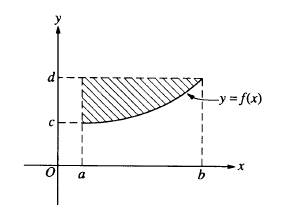
\includegraphics[width=2in]{original.jpg}
    \end{center}
    Which of the following represents the area of the shaded region in the figure above?

    $$\boxed{\int_{a}^{b} \big(d-f(x)\big)\,dx}$$

    \item A particle with velocity at any time $t$ given by $v(t)=e^t$ moves in a straight line. How far does the particle move from $t=0$ to $t=2$?

    $$\int_{0}^{2} v(t) \, dt = e^t \biggr\rvert_{0}^{2} = \boxed{e^2-1}$$
\newpage
    \item The furnace in a home consumes heating oil during a particular month at a rate modeled by the function $F$ given by $F(t)=0.3+0.1t-0.85\cos\big(\frac{2\pi}{15}(t+5)\big)$, where $F(t)$ is measured in gallons per day and $t$ is the number of days since the start of the month. How many gallons of oil does the furnace consume during the first 14 days of the month (from $t=0$ to $t=14$)?
    $$\int_{0}^{14} F(t) \, dt \approx \boxed{13.7392 \text{ gallons}}$$
    
    \item What is the area of the region in the first quadrant bounded on the left by the graph of $x=y^2$ and on the right by the graph of $x=4y-3$ for $1\leq y \leq3$?
    \begin{enumerate}
        \item $y^2=4y-3$ when $y=1$ and $y=3$.
    \end{enumerate}
    $$\int_{1}^{3} \big((4y-3)-y^2\big) \, dy = 2y^2-3y-\frac{y^3}{3}\biggr\rvert_{1}^{3} = \biggr(18-9-9\biggr) - \biggr(2-3-\frac{1}{3}\biggr) = \boxed{\frac{4}{3}}$$
    \item 
    \begin{center}
        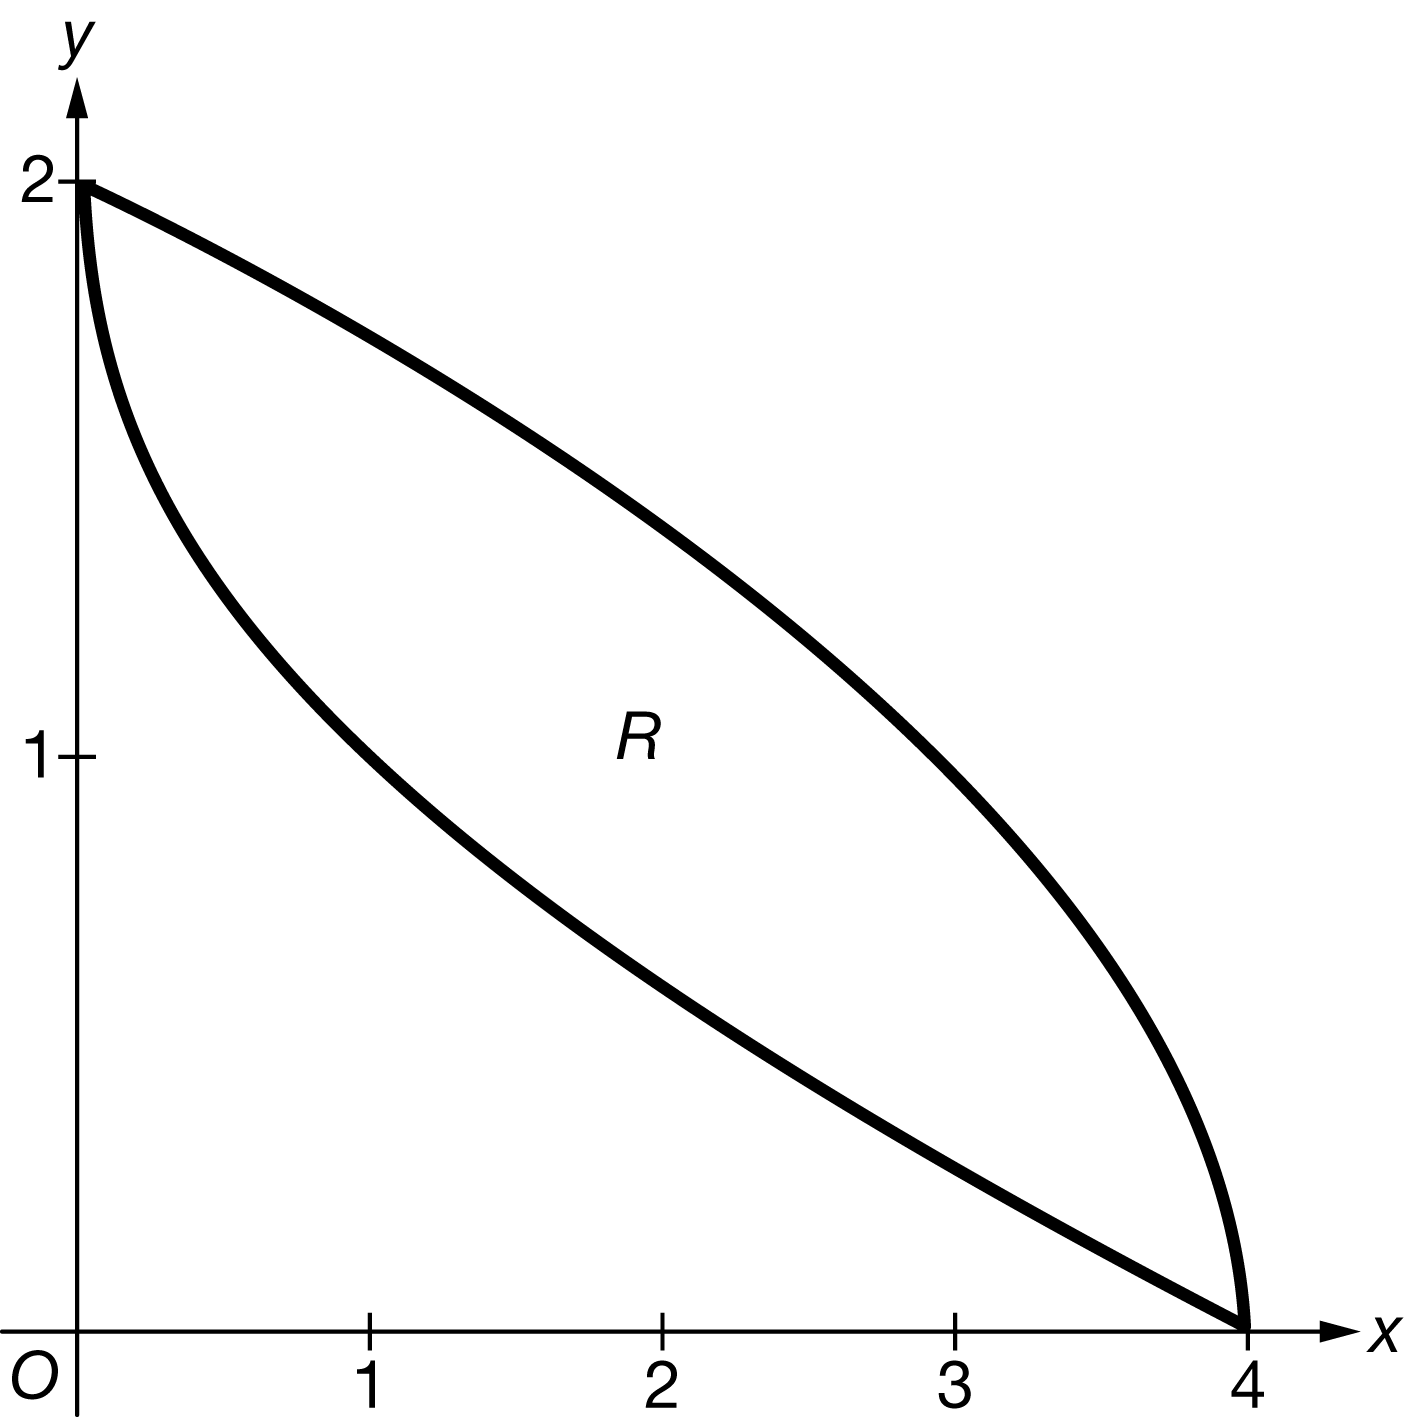
\includegraphics[width=2in]{4.011.png}
    \end{center}
    Let $R$ be the region in the first quadrant bounded above by the graph of $y=\frac{4}{\pi}\arccos\big( \frac{x}{4}\big)$ and below by the graph of $y=2-\sqrt{x}$, as shown in the figure above. What is the area of the region?
    $$R = \int_{0}^{4} \biggr(\frac{4}{\pi}\arccos\biggr( \frac{x}{4}\biggr) - \big(2-\sqrt{x}\big) \biggr) \, dx$$
$$\Longrightarrow \frac{4}{\pi}\int_{0}^{4} \arccos\biggr( \frac{x}{4}\biggr) \, dx + \int_{0}^{4} \big(2-\sqrt{x}\big) \, dx$$
\begin{enumerate}
    \item Let $w=\frac{x}{4} \Longrightarrow 4 dw=dx$
\end{enumerate}
$$\Longrightarrow \frac{16}{\pi}\int_{0}^{4} \arccos (w) \, dw \: + \: \biggr[2x-\frac{2}{3}x^{3/2} \biggr]_{0}^{4}$$
\begin{enumerate}[resume]
    \item Let $u=\arccos w \Longrightarrow  du=\frac{-1}{\sqrt{1-w^2}} \, dw$
    \item $dv=dw \Longrightarrow v=w$
\end{enumerate}
$$\Longrightarrow \frac{16}{\pi}\biggr[w \cdot \arccos w - \int \frac{-w}{\sqrt{1-w^2}} \, dw  \biggr]_{0}^{1} - \frac{8}{3}$$
\begin{enumerate}[resume]
\item Let $u= 1-w^2 \Longrightarrow \frac{1}{2} du = -w dw $
\end{enumerate}
$$\Longrightarrow\frac{16}{\pi}\biggr[w \cdot \arccos w - \frac{1}{2} \int u^{-1/2} \, du  \biggr]_{0}^{1} - \frac{8}{3}$$
$$\Longrightarrow\frac{16}{\pi}\biggr[w \cdot \arccos w  + \sqrt{1-w^2}  \biggr]_{0}^{1} - \frac{8}{3}$$
$$\Longrightarrow \boxed{\frac{16}{\pi}- \frac{8}{3}}$$
    
    \item Let $R$ be the region in the first quadrant bounded above by the graph of $y=1+4x$ and below by the graph of $y=3^x$ for $0 \leq x \leq 2$. Which of the following definite integrals gives the area of region $R$?
    \begin{enumerate}
        \item \textbf{Intersection:} $(0,1)$ and $(2,9)$
    \end{enumerate}
$$\int_{0}^{2} \big((1+4x)-(3^x) \big) \, dx = \int_{1}^{9} \bigg( \frac{\ln y}{\ln 3} - \frac{y-1}{4} \biggr)\, dy $$
$$\boxed{\text{I and III only}}$$


    \item What is the area of the region in the first quadrant bounded on the left by the graph of $\frac{y^2}{2}$ and on the right by the graph of $x=3y-4$ for $2 \leq x \leq 4$?
    \begin{enumerate}
        \item \textbf{Intersection:} $(2,2)$ and $(8,4)$
    \end{enumerate}
    $$\int_{2}^{4} \biggr((3y-4)-(\frac{y^2}{2}) \biggr) \,dy = \biggr[ \frac{3y^2}{2}-4y-\frac{y^3}{6}\biggr]_{2}^{4} = \biggr(24-16-\frac{64}{6}\biggr) - \biggr(6-8-\frac{8}{6}\biggr)= \boxed{10-\frac{56}{6}}$$
    
    \item 
    \begin{center}
        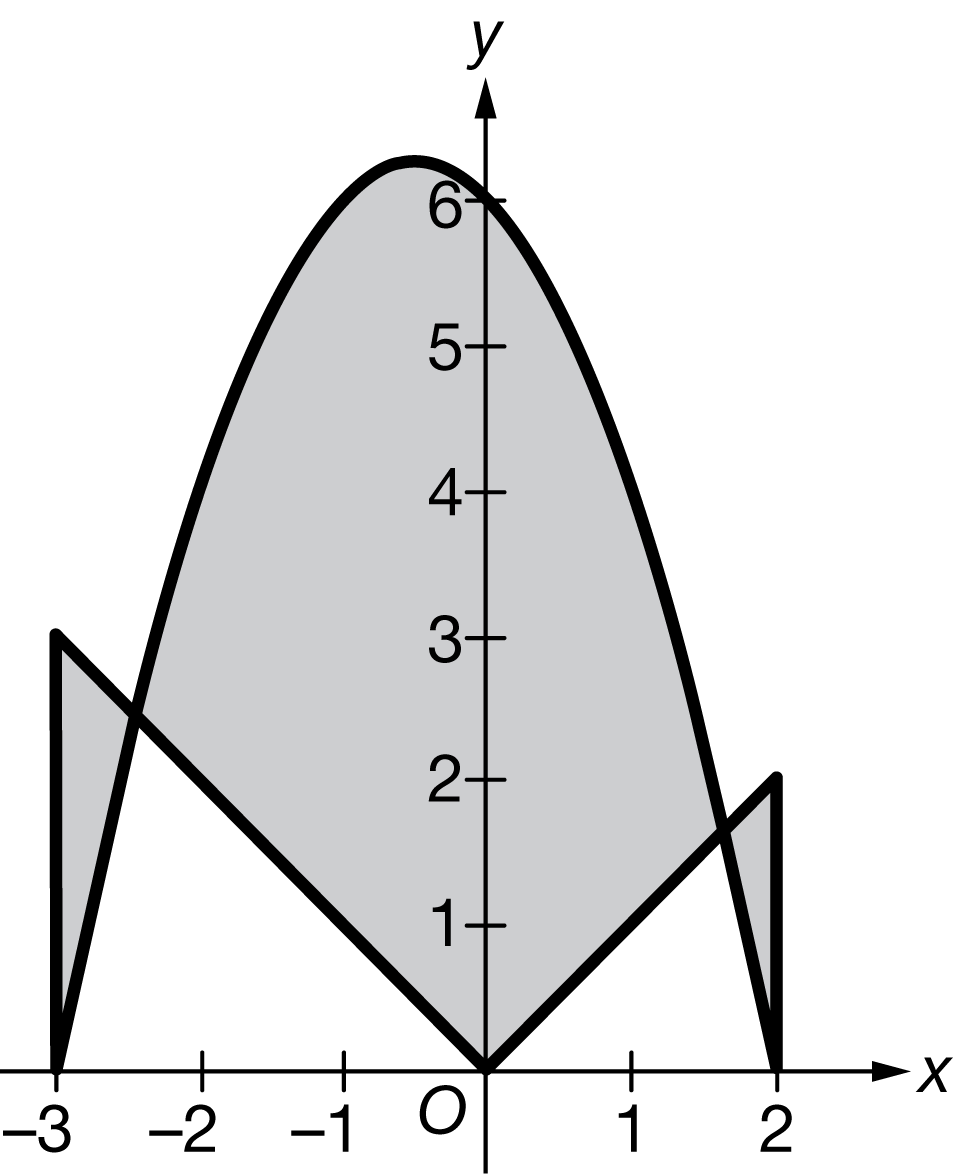
\includegraphics[width=2in]{4.012.png}
    \end{center}
    The figure above shows the graphs of $y=|x|$ and $y=6-x-x^2$ for $-3 \leq x \leq 2$. The $x$-coordinates of the points of intersection of the graphs are $x_1$ and $x_2$, where $x_1<x_2$. Which of the following gives the sum of the areas of the shaded regions?
    $$\boxed{\int_{-3}^{x_1}\big(|x|-(6-x-x^2)\big) \,dx + \int_{x_1}^{x_2}\big( (6-x-x^2)-|x|\big)\,dx + \int_{x_2}^{2}\big(|x|-(6-x-x^2)\big) \,dx}$$

\end{enumerate}
\section*{4.02}
\begin{enumerate}
    \item 
    \begin{center}
        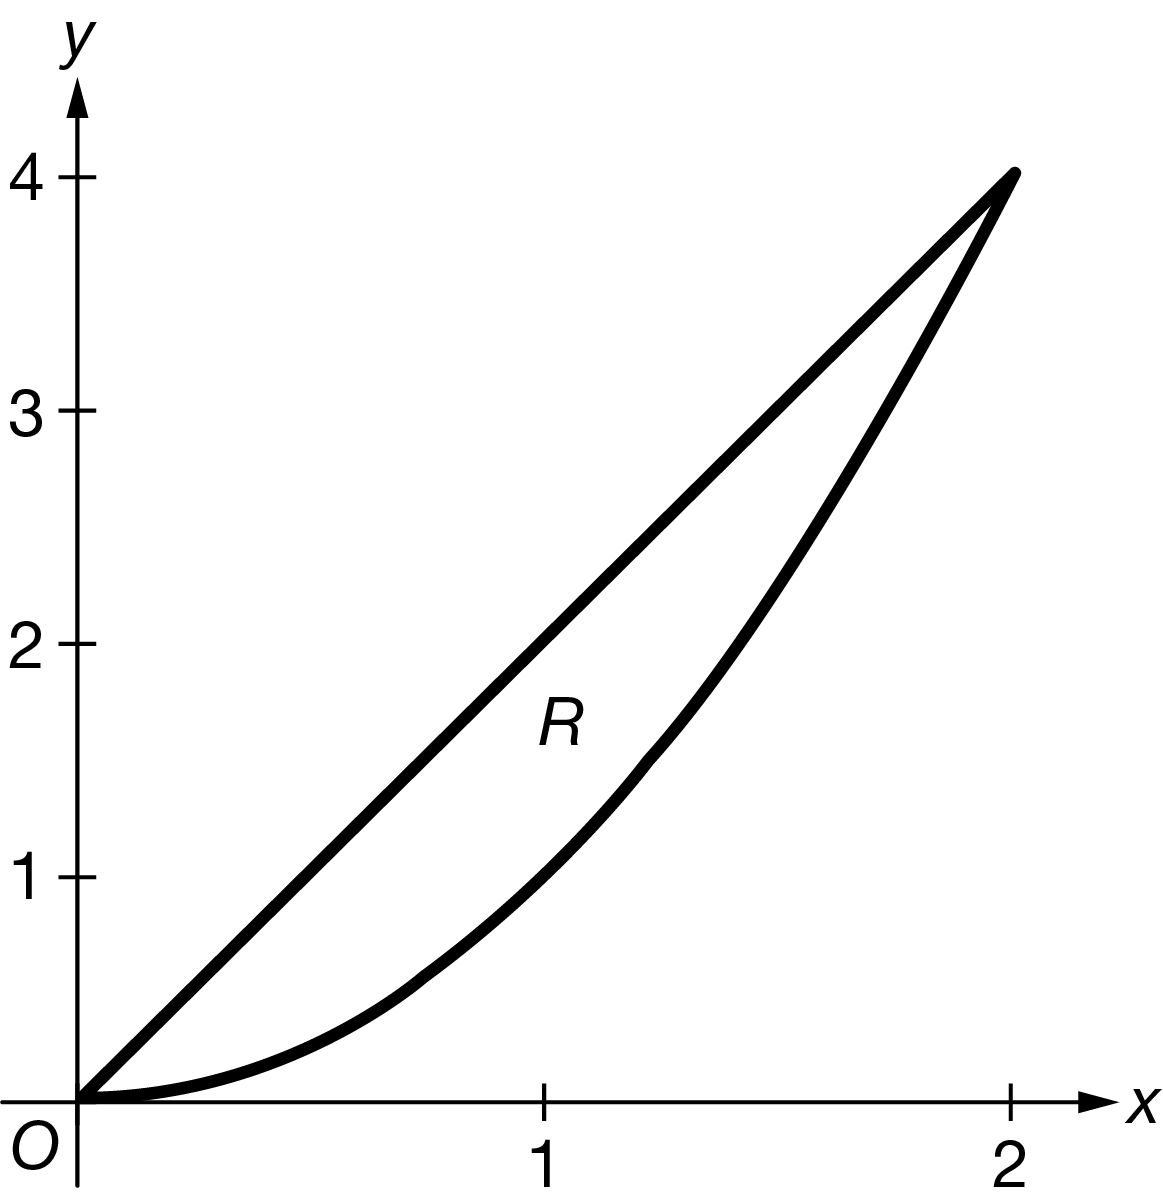
\includegraphics[width=2in]{4.021.png}
    \end{center}
    Let $R$ be the region in the first quadrant bounded by the graphs of $y=x^2$ and $y=2x$, as shown in the figure above. The region $R$ is the base of a solid. For the solid, each cross section perpendicular to the $y$-axis is a square. What is the volume of the solid?
    \begin{enumerate}
        \item $y=x^2 \Longrightarrow \sqrt{y}=x$
        \item $y=2x \Longrightarrow \frac{y}{2}=x$
    \end{enumerate}
    $$V=\int_{0}^{4} \biggr( \sqrt{y} - \frac{y}{2}\biggr)^2 \, dy = \frac{8}{15} \approx \boxed{0.533}$$
    \item The base of a solid is the region in the first quadrant bounded by the graph of $y=\cos x$ and the $x$- and $y$-axes for $0 \leq x \leq \frac{\pi}{2}$. For the solid, each cross section perpendicular to the $y$-axis is a rectangle whose height is four times its width in the $xy$-plane. What is the volume of the solid?
    \begin{enumerate}
        \item $y=\cos x \Longrightarrow \arccos y = x$
        \item $\cos \big(\frac{\pi}{2}\big) = 0$ and $\cos \big(0\big)=1$
    \end{enumerate}
    $$V=4 \cdot \int_{0}^{1} \arccos^2 y \, dy =\pi-2 \approx \boxed{4.566}$$

    \item The base of a solid is the region in the first quadrant between the graph of $y=x^2$ and the $x$-axis for $0 \leq x \leq 1$. For the solid, each cross section perpendicular to the $x$-axis is a quarter circle with the corresponding circle’s center on the $x$-axis and one radius in the $xy$-plane. What is the volume of the solid?
    \begin{enumerate}
        \item $A=\frac{\pi r^2}{4}$ 
        \item $x^2-0= r \Longrightarrow A = \frac{\pi}{4} x^2$
    \end{enumerate}
    $$V=\frac{\pi}{4} \cdot \int_{0}^{1} x^4 \, dx = \frac{\pi}{4}\cdot \frac{x^5}{5}\biggr\rvert_{0}^{1} = \boxed{\frac{\pi}{20}}$$
\newpage
    \item The base of a solid is the region in the first quadrant between the graph of $y=x^2$ and the $x$-axis for $0 \leq x \leq 1$. For the solid, each cross section perpendicular to the $x$-axis is a semicircle. What is the volume of the solid?
    $$V=\frac{\pi}{8}\cdot \int_{0}^{1} x^4 \, dx = \frac{\pi}{8} \cdot \frac{x^5}{5}\biggr\rvert_{0}^{1} =\boxed{ \frac{\pi}{40}}$$

    \item Let $R$ be the region in the first quadrant bounded by the graph of $y=x^3$, the line $x=2$, and the $x$-axis. $R$ is the base of a solid whose cross sections perpendicular to the $x$-axis are equilateral triangles. What is the volume of the solid?

    $$V=\frac{\sqrt{3}}{4} \cdot \int_{0}^{2} (x^3)^2 \, dx = \frac{\sqrt{3}}{4} \cdot \frac{x^7}{7}\biggr\rvert_{0}^{2} = \frac{\sqrt{3}}{4} \cdot \frac{128}{7} = \frac{128\sqrt{3}}{28}=\boxed{\frac{32\sqrt{3}}{7}}$$
    
    \item The base of a solid is the region in the first quadrant bounded by the graph of $y=2-\frac{2x}{3}$ and the $x$- and $y$-axes for $0 \leq x \leq 3$. For the solid, each cross section perpendicular to the $y$-axis is a rectangle whose height is five times its width in the $xy$-plane. What is the volume of the solid?
    \begin{enumerate}
        \item $y=2-\frac{2x}{3} \Longrightarrow x=\frac{6-3y}{2}$
    \end{enumerate}
    $$V=5 \cdot \int_{0}^{3} \biggr(\frac{6-3y}{2}\biggr)^2 \, dx= \boxed{30.00}$$
    
    \item The base of a solid is the region in the first quadrant bounded by the graph of $y=1-\frac{x}{3}$ and the $x$- and $y$-axes. For the solid, each cross section perpendicular to the $x$-axis is a square. What is the volume of the solid?
    $$V=\int_{0}^{3} \biggr( 1-\frac{x}{3}\biggr) \, dx = \int_{0}^{3} \biggr( \frac{x^2}{9} - \frac{2x}{3} + 1\biggr) \, dx = \biggr[\frac{x^3}{27}-\frac{x^2}{3}+x\biggr]_{0}^{3} = 1-3+3 =\boxed{1.00}$$

    \item The region bounded by the graph of $y=2x-x^2$ and the $x$-axis is the base of a solid. For this solid, each cross section perpendicular to the $x$-axis is an equilateral triangle. What is the volume of the solid?
    $$V=\frac{\sqrt{3}}{4} \cdot \int_{0}^{2} \biggr( 2x-x^2\biggr)^2 \, dx = \frac{4\sqrt{3}}{15}\approx \boxed{0.462}$$

    \item The base of a solid is the region enclosed by the curve $\frac{x^4}{16}+\frac{y^4}{81}=1$ shown in the figure above. For the solid, each cross section perpendicular to the $x$-axis is a semicircle. What is the volume of the solid?
    \begin{enumerate}
        \item $\frac{x^4}{16}+\frac{y^4}{81}=1 \Longrightarrow y=\pm \sqrt[4]{81-\frac{81x^4}{16}}$
    \end{enumerate}
    $$V=\frac{\pi}{8}\cdot \int_{-2}^{2} \Biggr( 2 \cdot \sqrt[4]{81-\frac{81x^4}{16}}\Biggr)^2 \, dx \approx\boxed{49.425} $$
\newpage
    \item 
    \begin{center}
        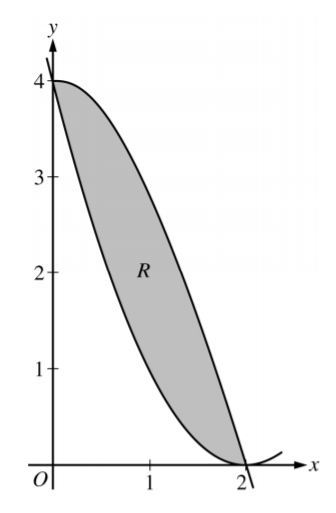
\includegraphics[width=1.5in]{original-27.png}
    \end{center}
    Let $R$ be the region in the first quadrant bounded by the graphs of $y=4\cos \big(\frac{\pi x}{4}\big)$ and $y=(x-2)^2$, as shown in the figure above. The region $R$ is the base of a solid. For the solid, each cross section perpendicular to the $x$-axis is an isosceles right triangle with a leg in region $R$. What is the volume of the solid?
    $$V=\frac{1}{2}\cdot \int_{0}^{2} \biggr(4\cos \biggr(\frac{\pi x}{4}\biggr)- (x-2)^2\biggr)^2 \, dx =\frac{8\cdot (7\pi^3-160\pi +320)}{5\pi^3} \approx \boxed{1.775}$$

    \item Let $R$ be the region in the first quadrant bounded by the $y$-axis, the $x$-axis, the graph of $y=e^{\frac{-x^2}{2}}$, and the line $x=3$. The region $R$ is the base of a solid. For the solid, each cross section perpendicular to the $x$-axis is a square. What is the volume of the solid?
    $$V=\int_{0}^{3} \biggr(e^{\frac{-x^2}{2}}\biggr) \, dx = \int_{0}^{3} e^{-x^2} \, dx \approx \boxed{0.886} $$
    \item Let $R$ be the region in the first quadrant bounded below by the graph of $y=x^2$ and above by the graph of $y=\sqrt{x}$. $R$ is the base of a solid whose cross sections perpendicular to the $x$-axis are squares. What is the volume of the solid?
    \begin{enumerate}
        \item $x^2=\sqrt{x}$ when $x=0$ and $x=1$
    \end{enumerate}
    $$V=\int_{0}^{1} \biggr(\sqrt{x}-x^2\biggr)^2\, dx =\frac{9}{70} \approx \boxed{0.129}$$

    \item Let $R$ be the region in the first quadrant bounded above by the graph of $y=\ln(3-x)$, for $0 \leq x \leq 2$. $R$ is the base of a solid for which each cross section perpendicular to the $x$-axis is a square. What is the volume of the solid?

    $$V=\int_{0}^{2} \ln^2(3-x) \, dx = 3\ln^2(3)-6\ln(3)+4 \approx \boxed{1.029}$$

    \item
    \begin{center}
        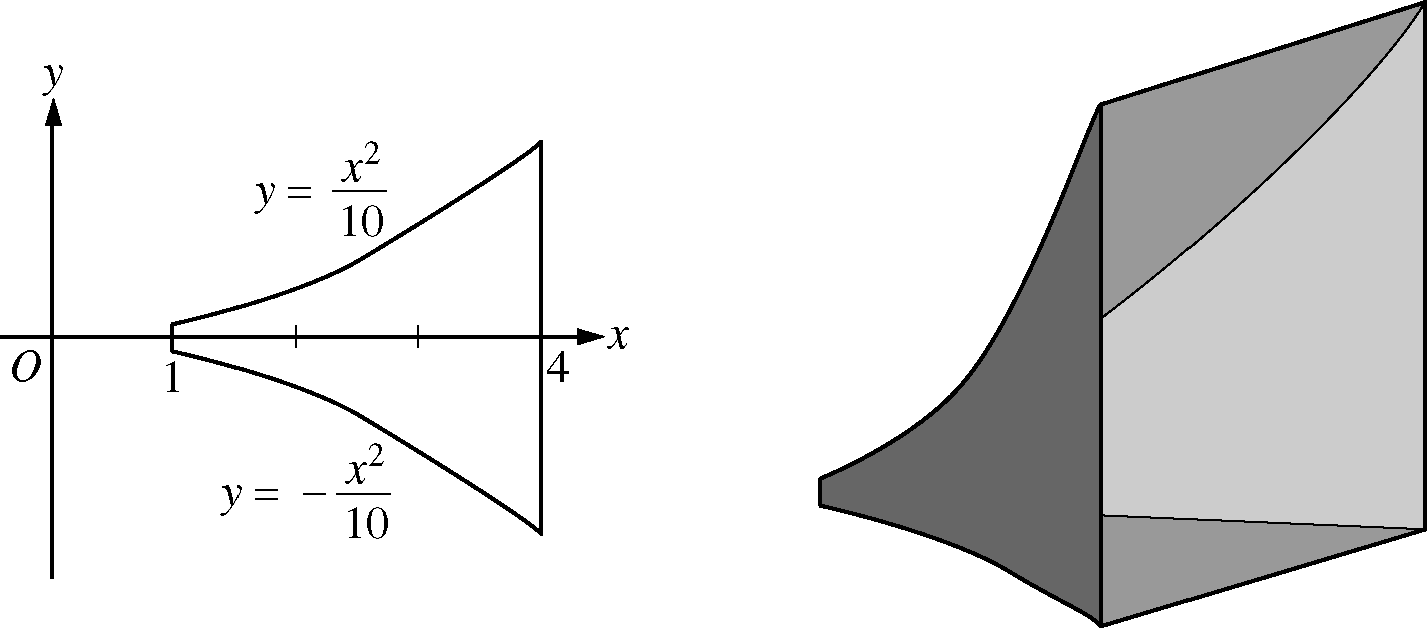
\includegraphics[width=4in]{4.022.png}
    \end{center}
    The base of a loudspeaker is determined by the two curves $y=\frac{x^2}{10}$ and $y=- \frac{x^2}{10}$ for as shown in the figure above. For this loudspeaker, the cross sections perpendicular to the $x$-axis are squares. What is the volume of the loudspeaker, in cubic units?
$$V=\int_{0}^{4} \biggr(\frac{x^2}{10}\biggr)^2 \, dx  = \int_{0}^{4} \frac{x^4}{25} \, dx = \frac{1023}{125} = \boxed{8.184}$$
    \item The base of a solid is the region in the first quadrant enclosed by the parabola $y=4x^2$, the line $x=1$, and the $x$-axis. Each plane section of the solid perpendicular to the $x$-axis is a square. The volume of the solid is

    $$V=\int_{0}^{1} \big(4x^2\big)^2 \, dx = \int_{0}^{1} 16x^4 \, dx = \frac{16x^5}{5}\biggr\rvert_{0}^{1}=\boxed{\frac{16}{5}}$$

\end{enumerate}
\section*{4.03}
\begin{enumerate}
    \item Let $S$ be the region enclosed by the graphs of $y = 2x$ and $y = 2x^2$ for $0 \leq x \leq 1$. What is the volume of the solid generated when $S$ is revolved about the line $y = 3$?
    \begin{enumerate}
        \item $2x=2x^2$ when $x=0$ and $x=1$
        \item $R(x)=(3-2x^2)$
        \item $r(x)=(3-2x)$
    \end{enumerate}
    $$\boxed{V=\pi\int_0^1\biggr((3-2x^2)^2-(3-2x)^2\biggr) \, dx}$$

    \item What is the volume of the solid generated when the region in the first quadrant bounded by the graph of $y=e^x$, the $x$-axis, and the vertical line $x=\ln 2$ is revolved about the $x$-axis?
   $$V=\pi\int_{0}^{\ln 2} \big(e^x\big)^2 \, dx = \pi\int_{0}^{\ln 2} e^{2x}\, dx = \frac{\pi}{2} e^{2x} \biggr\rvert_{0}^{\ln 2} \, dx = \frac{\pi}{2}\biggr(4-1\biggr) =\boxed{ \frac{3\pi}{2} }$$
\newpage
    \item 
    \begin{center}
        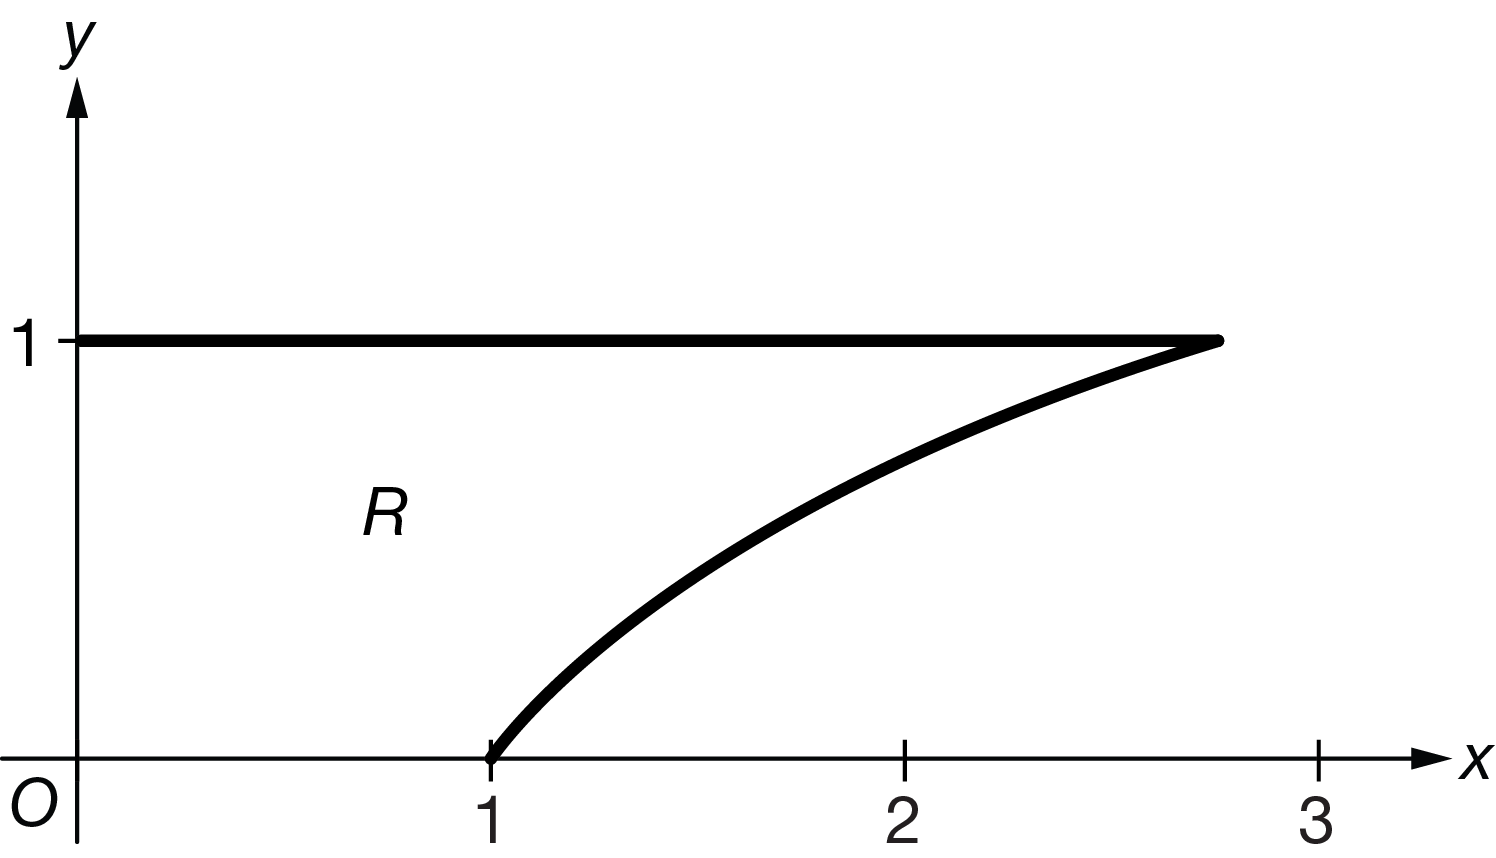
\includegraphics[width=2in]{4.031.png}
    \end{center}
    Let $R$ be the region in the first quadrant bounded by the $x$- and $y$-axes, the horizontal line $y=1$, and the graph of $y=\ln x$, as shown in the figure above. What is the volume of the solid generated when region $R$ is revolved about the $y$-axis?
    \begin{enumerate}
        \item $y=\ln x \Longrightarrow x = e^y$
    \end{enumerate}
    $$V=\pi\int_{0}^{1} \big(e^y\big)^2 \, dy = \pi\int_{0}^{1} e^{2x}\, dy = \frac{\pi}{2} e^{2y} \bigg\rvert_{0}^{1} \, dy = \boxed{\frac{\pi\big(e^2-1\big)}{2}}$$

    \item Let $R$ be the triangular region in the first quadrant with vertices at points $(0,0)$, $(h,0)$, and $(h,r)$, where $r$ and $h$ are positive constants. Which of the following gives the volume of the solid generated when region $R$ is revolved about the $x$-axis?
    \begin{enumerate}
        \item $m=\frac{y_2-y_1}{x_2-x_1} = \frac{r-0}{h-0}=\frac{r}{h}$
        \item $y=\frac{r}{h}\cdot x$
    \end{enumerate}
    $$\boxed{V=\pi\int_{0}^{h} \biggr(\frac{r}{h}\cdot x\biggr)^2 \, dx}$$
    \item 
    \begin{center}
        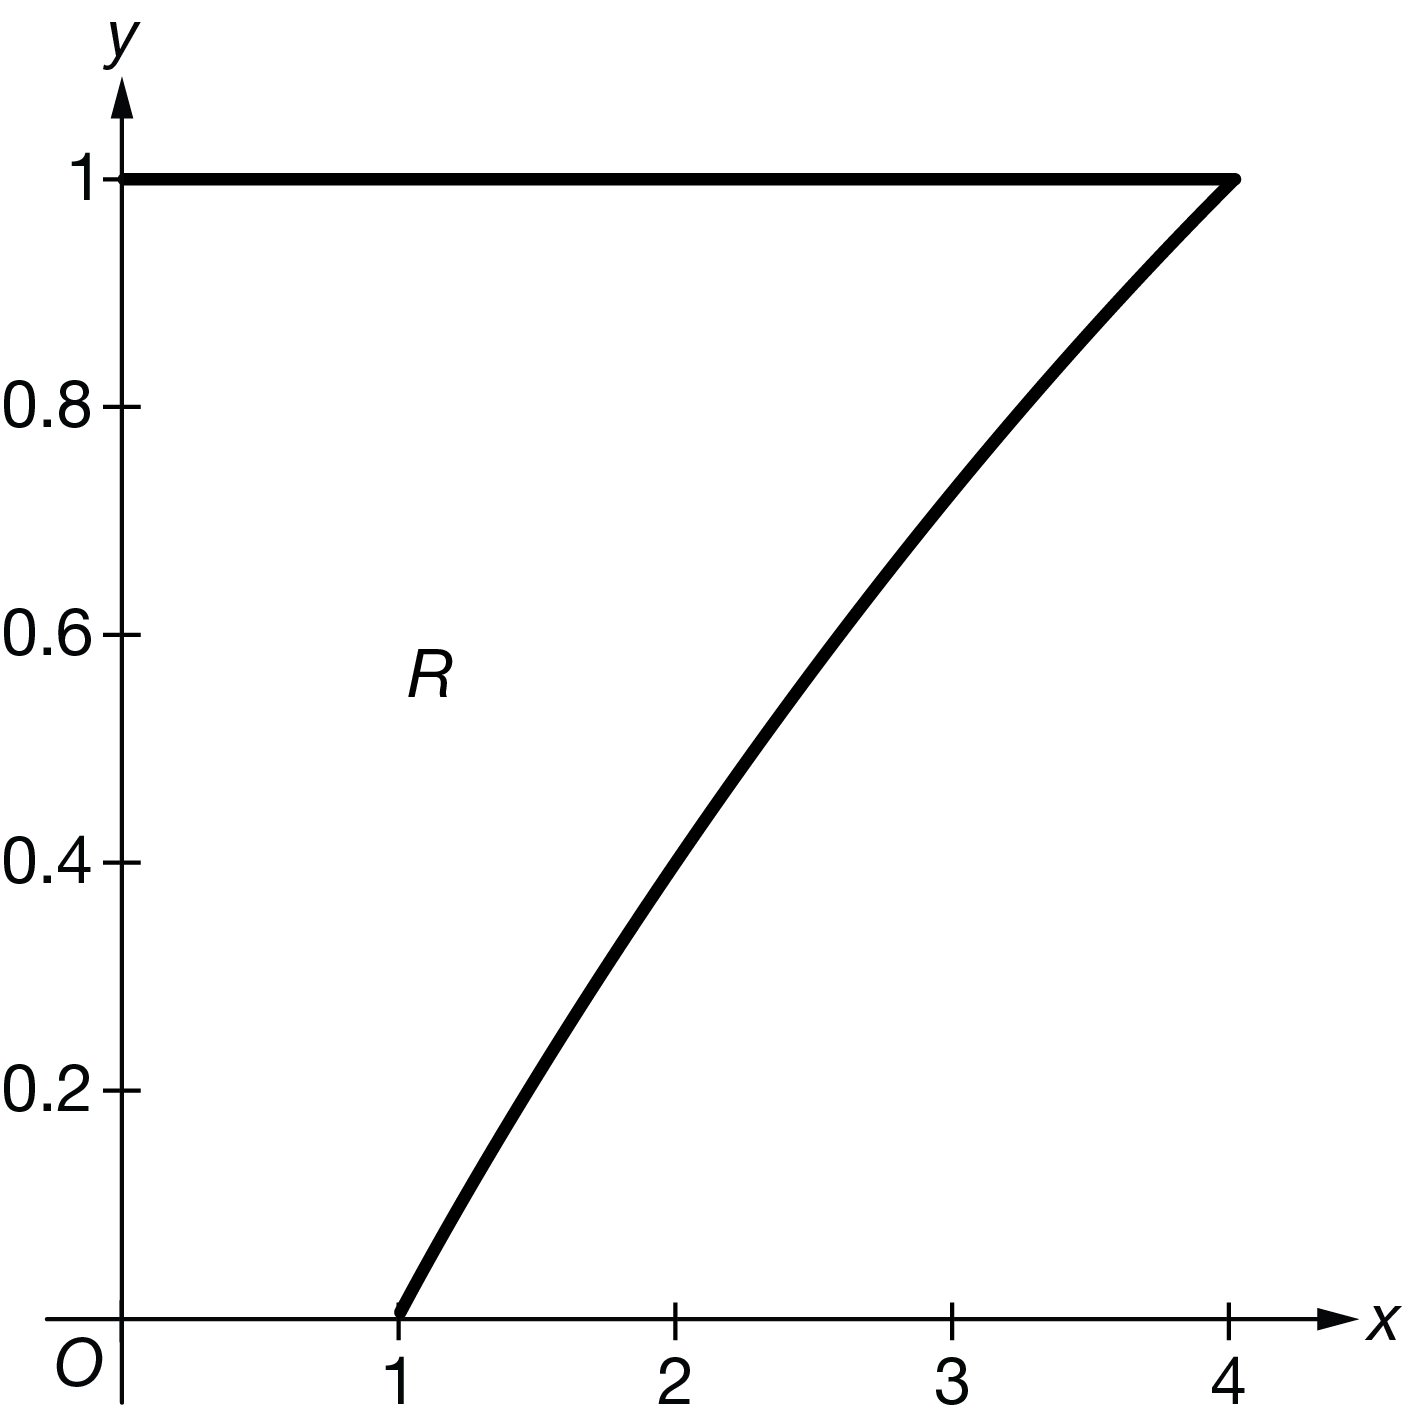
\includegraphics[width=2in]{4.032.png}
    \end{center}
    Let $R$ be the region in the first quadrant bounded by the $x$- and $y$-axes, the horizontal line $y=1$, and the graph of $y=\sqrt{x}$, as shown in the figure above. What is the volume of the solid generated when region $R$ is revolved about the $y$-axis?
    \begin{enumerate}
        \item $y=\sqrt{x} \Longrightarrow x=(y+1)^2$
    \end{enumerate}
    $$V=\pi\int_{0}^{1} \biggr((y+1)^2\biggr)^2 \, dy =\pi\int_{0}^{1} (y+1)^4 \, dy $$
    \begin{enumerate}
        \item Let $u=y+1 \Longrightarrow du=dy$
    \end{enumerate}
    $$V=\pi\int_{1}^{2} u^4 \, du = \pi \frac{x^5}{5} \biggr\rvert_{1}^{2} = \pi \biggr(\frac{32}{5}-\frac{1}{5}\biggr) = \boxed{\frac{31\pi}{5}}$$

    \item Let $R$ be the triangular region in the first quadrant with vertices at points $(0,0)$, $(a,0)$, and $(0,b)$, where $a$ and $b$ are positive constants. Which of the following gives the volume of the solid generated when region $R$ is revolved about the $x$-axis?
    \begin{enumerate}
        \item $m=\frac{y_2-y_1}{x_2-x_1} = \frac{0-b}{a-0}=\frac{-b}{a}$
        \item $y=\frac{-b}{a}x+b$
    \end{enumerate}
    $$\boxed{V=\pi\int_{0}^{a}\biggr(\frac{-b}{a}x+b\biggr) \, dx}$$

    \item What is the volume of the solid generated when the region bounded by the graph of $y=x^2$, the vertical line $x=3$, and the horizontal line $y=4$ is revolved about the horizontal line $y=4$?
    \begin{enumerate}
        \item $4=x^2 \Longrightarrow x=\pm 2$
        \item $(2,4)$ and $(3,9)$
    \end{enumerate}
    $$\boxed{V=\pi\int_{2}^{3} \big(x^2-4\big)^2 \, dx}$$

    \item What is the volume of the solid generated when the region bounded by the graph of $y=2x,$ the horizontal line $y=2$, and the $y$-axis is revolved about the horizontal line $y=2$?
    $$V=\pi\int_{0}^{1} \big(2-2x\big)^2 \, dx =\pi\int_{0}^{1} \big(4x^2-8x+4\big) \, dx=\pi\biggr[\frac{4x^3}{3}-4x^2+4x\biggr]_{0}^{1} = \boxed{\frac{4\pi}{3}}$$
   

    \item Let $R$ be the region in the first quadrant bounded by the graph of $y=\sin x$, the $x$-axis, and the vertical line $x=1$. Which of the following gives the volume of the solid generated when region $R$ is revolved about the vertical line $x=1$ ?
    \begin{enumerate}
        \item $y =\sin x \Longrightarrow x=\arcsin y$
    \end{enumerate}
    $$\boxed{V=\pi\int_{0}^{\sin 1} \big(1-\arcsin y\big)^2 \, dy}$$

    \item What is the volume of the solid generated when the region bounded by the graph of $y=x^3$, the vertical line $x=4$, and the horizontal line $y=8$ is revolved about the horizontal line $y=8$?
    $$\boxed{V=\pi \int_{0}^{4}\big(x^3-8\big)^2 \, dx}$$

    \item 
    \begin{center}
        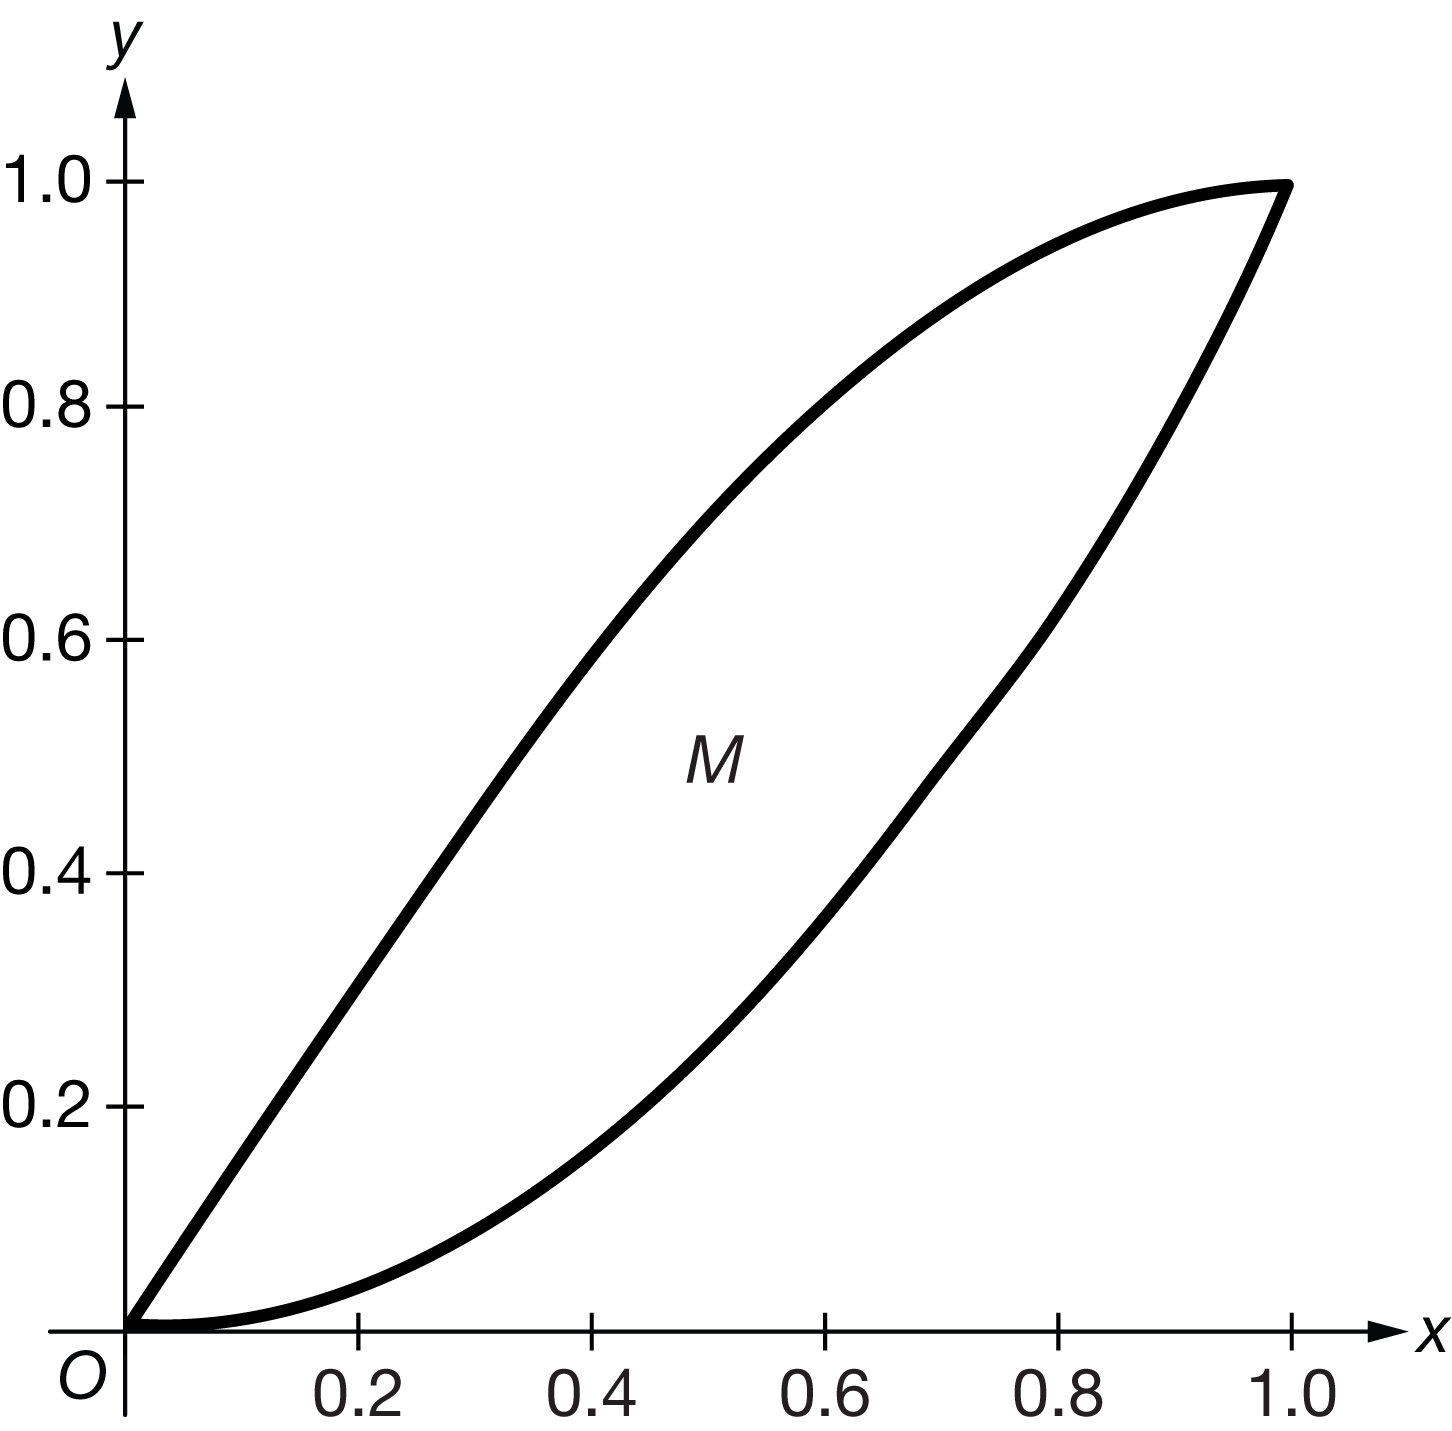
\includegraphics[width=2in]{4.033.png}
    \end{center}
    Let $M$ be the region in the first quadrant bounded by the graphs of $y=\sin\big(\frac{\pi x}{2}\big)$ and $y=x^2$. What is the volume of the solid generated when region $M$ is revolved around the vertical line $x=2$?
    \begin{enumerate}
        \item $y=\sin\big(\frac{\pi x}{2}\big) \Longrightarrow x=\frac{2\arcsin(y)}{\pi}$
        \item $y=x^2 \Longrightarrow x=\sqrt{y}$
    \end{enumerate}
    $$V=\pi\int_{0}^{1} \Biggr(\biggr(2-\frac{2\arcsin(y)}{\pi}\biggr)^2-\big(2-\sqrt{y}\big)^2 \Biggr) \, dy = \frac{-(5\pi^2-48\pi+48)}{6\pi}\approx \boxed{2.836}$$

    \item What is the volume of the solid generated when the circular region bounded by the graph of $x^2+y^2=1$ is revolved around the horizontal line $y=3$?
    $$V=\pi \int_{-1}^{1} \Biggr(\bigg(3+\sqrt{1-x^2}\bigg)^2-\bigg(3-\sqrt{1-x^2}\bigg)^2\Biggr) \, dx$$
    \begin{enumerate}
        \item $\bigg(3+\sqrt{1-x^2}\bigg)^2 = 9+6\sqrt{1-x^2}+(1-x^2)$ 
        \item $\bigg(3-\sqrt{1-x^2}\bigg)^2 = 9-6\sqrt{1-x^2}+(1-x^2)$ 
    \end{enumerate}
    $$V=12\pi\int_{-1}^{1} \biggr(\sqrt{1-x^2}\biggr) \, dx$$
    \begin{enumerate}[resume]
        \item Let $x=\sin \theta \Longrightarrow dx = \cos \theta \, d\theta$
    \end{enumerate}
    $$V=12\pi\int_{\arcsin(-1)}^{\arcsin(1)} \sqrt{1-\sin^2 \theta} \cdot \cos\theta \, d\theta$$
    \begin{enumerate}[resume]
        \item $1-\sin\theta = \cos^2 \theta$
    \end{enumerate}
     $$V=12\pi\int_{\frac{-\pi}{2}}^{\frac{\pi}{2}} \cos^2 \theta \, d\theta$$
\begin{enumerate}[resume]
        \item $\cos^2 \theta = \frac{1}{2}\biggr(1+\cos(2\theta)\biggr)$
    \end{enumerate}
 $$V=6\pi\int_{\frac{-\pi}{2}}^{\frac{\pi}{2}} \biggr(1+\cos(2\theta)\biggr) \, d\theta$$
 $$V=6\pi\biggr[\theta +\frac{\sin (2\theta)}{2}\biggr]_{\frac{-\pi}{2}}^{\frac{\pi}{2}}=6\pi\Biggr[\bigg(\frac{\pi}{2}+\frac{\sin \pi}{2}\bigg)-\bigg(\frac{-\pi}{2}+\frac{\sin (-\pi)}{2}\bigg)\Biggr] =\boxed{ 6\pi^2}$$
    
    \item 
    \begin{center}
        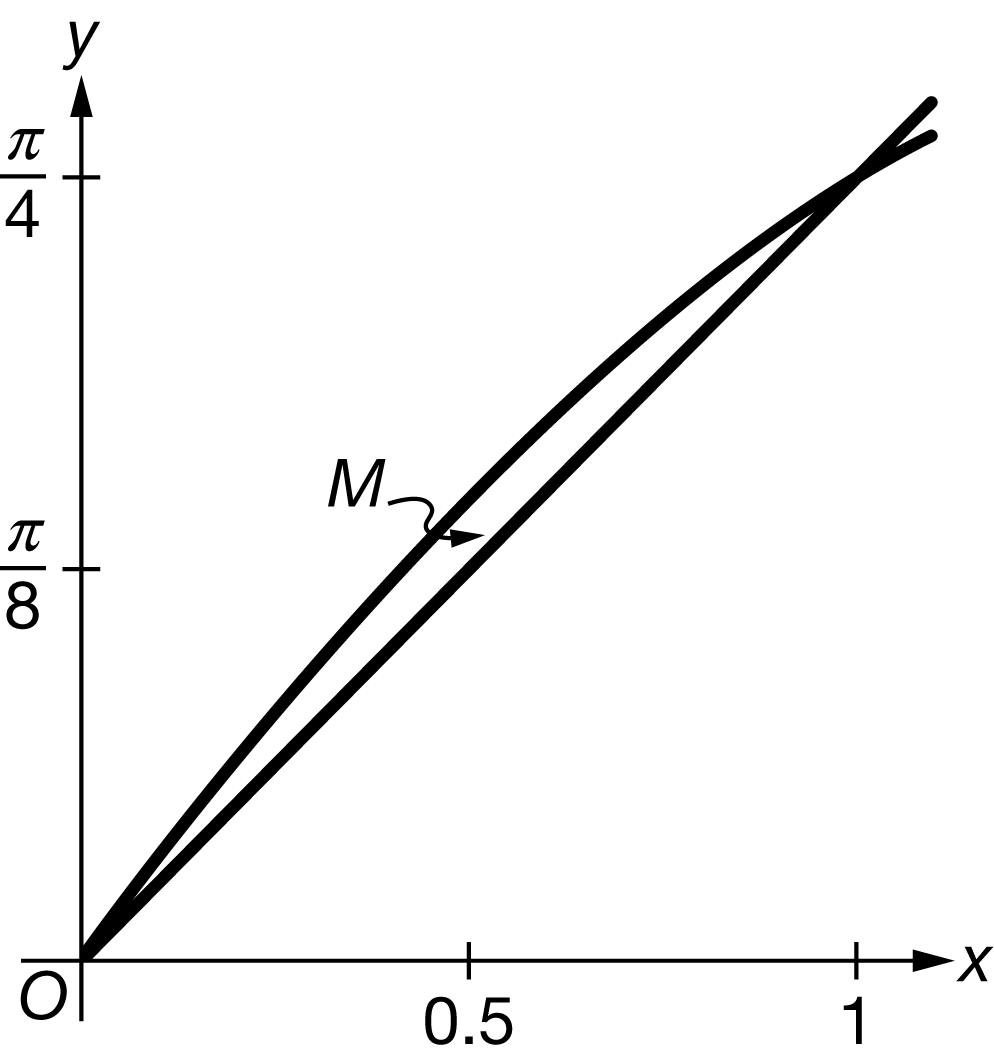
\includegraphics[width=2in]{4.034.png}
    \end{center}
    Let $M$ be the region in the first quadrant bounded by the graphs of $y=\arctan x$ and $y=\frac{\pi}{4}x$, as shown in the figure above. What is the volume of the solid generated when region $M$ is revolved around the vertical line $x=2$?
    \begin{enumerate}
        \item $y=\arctan x \Longrightarrow x =tan y$
        \item $y=\frac{\pi x}{4} \Longrightarrow x= \frac{4y}{\pi}$
    \end{enumerate}
    $$V=\pi\int_{0}^{\frac{\pi}{4}} \Biggr(\big(2-\tan y\big)^2 -\big(2-\frac{4y}{\pi}\big)^2\biggr)\, dy = \frac{-\pi(12\ln(2)-\pi-6)}{6}\approx \boxed{0.431}$$
    \begin{center}
        \textbf{OR}
    \end{center}
    $$V=\int_{0}^{2\pi}\int_{0}^{\frac{\pi}{4}}\int_{2-\frac{4y}{\pi}}^{2-\tan y} r \, dt\, dy\, d\theta \approx \boxed{0.431}$$
    
    \item 
    \begin{center}
        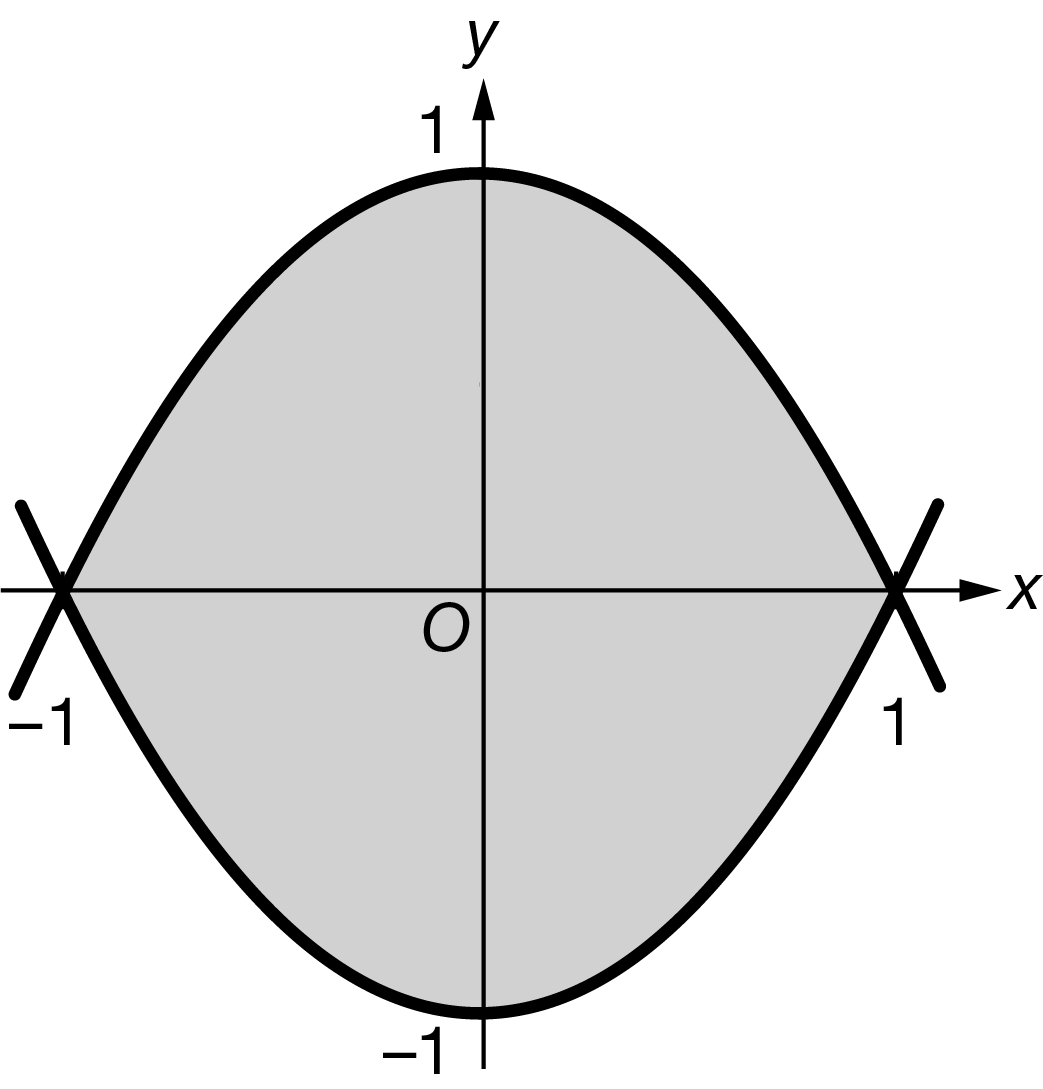
\includegraphics[width=2in]{4.035.png}
    \end{center}
    Let $R$ be the region bounded above by the graph of $y=1-x^2$ and below by the graph of $y=x^2-1$, for $-1 \leq x \leq 1$, as shaded in the figure above. What is the volume of the solid generated when region $R$ is revolved about the horizontal line $y=3$?
    $$V=\pi\int_{-1}^{1} \biggr(\big(3-(x^2-1)\big)^2-\big(3-(1-x^2)\big)^2\biggr) \, dx = \pi\int_{-1}^{1} \biggr(\big(4-x^2\big)^2-\big(2+x^2\big)^2\biggr) \, dx$$
    \begin{enumerate}
        \item $(4-x^2)=16-8x^2+x^4$
        \item $(2+^2)=4+4x^2+x^4$
    \end{enumerate}
    $$V=\pi\int_{-1}^{1} \bigg(12-12x^2\bigg) \, dx = \pi\biggr[12x-4x^3\biggr]_{-1}^{1} = \boxed{16\pi}$$

    \item The region in the first quadrant bounded by the graph of $y=\sec x$, $x=\frac{\pi}{4}$ and the axes is rotated about the $x$-axis. What is the volume of the solid generated?
    $$V=\pi\int_{0}^{\frac{\pi}{4}} \sec^2 x \, dx = \pi \tan x \biggrevert_{0}^{\frac{\pi}{4}} =pi(1-0) =\boxed{\pi}$$
\end{enumerate}
\section*{4.04}
\begin{enumerate}
    \item 
        \begin{table}[h]
        \centering
        \begin{tabular}{|l||l|l|l|l|}
        \hline
        $x$ & 1 & 3 & 5 & 7 \\ \hline
        $f(x)$ & 4 & 6 & 7 & 5 \\ \hline
        $f'(x)$ & 2 & 1 & 0 & -1 \\ \hline
        \end{tabular}
        \end{table}
        The table above gives selected values for a differentiable function $f$ and its first derivative. Using a left Riemann sum with 3 subintervals of equal length, which of the following is an approximation of the length of the graph of $f$ on the interval $[1,7]$?
$$s=\int_{1}^{7}\sqrt{1+(f'(x))^2} \, dx = \lim_{x\to\infty}\sum_{k=1}^{n} \sqrt{1+(f'(x_k))^2} \,  \Delta x$$
\begin{enumerate}
    \item Let $\Delta x = 2$
\end{enumerate}
$$\Longrightarrow s \approx  2\sqrt{1+(f'(1))^2} + 2 \sqrt{1+(f'(3))^2} + 2\sqrt{1+(f'(5))^2} = \boxed{2\sqrt{5}+2\sqrt{2}+2}$$
        \item Which of the following integrals gives the length of the curve $y=\ln x$ from $x=1$ to $x=2$?
        \begin{enumerate}
            \item $y=\ln x \Longrightarrow \frac{dy}{dx} = \frac{1}{x}$
        \end{enumerate}
        $$s= \int_{1}^{2} \sqrt{1+\bigg(\frac{dy}{dx}\bigg)^2} \, dx = \int_{1}^{2} \sqrt{1+\bigg(\frac{1}{x}\bigg)^2} \, dx= \boxed{\int_{1}^{2} \sqrt{1+\frac{1}{x^2}}\, dx}$$

        \item Which of the following integrals gives the length of the graph $y=\sin \big( \sqrt{x} \big)$ between $x = a$ and $x = b$, where $0 < a < b$?
        \begin{enumerate}
            \item $y= \cos(\sqrt{x}) \Longrightarrow \frac{dy}{dx} = \frac{\cos(\sqrt{x})}{2\sqrt{x}}$
        \end{enumerate}
        $$s=\int_{a}^{b}\sqrt{1+\bigg(\frac{dy}{dx}\bigg)^2}\,dx=\int_{a}^{b}\sqrt{1+\bigg(\frac{\cos(\sqrt{x})}{2\sqrt{x}}\bigg)^2}\, dx = \boxed{\int_{a}^{b} \sqrt{1+\frac{\cos^2(\sqrt{x})}{4x}} \, dx}$$
\newpage
        \item The length of the curve $y=\ln ( \sec x)$ from $x=0$ to $x=b$, where $0<b<\frac{\pi}{2}$, may be expressed by which of the following integrals?
        \begin{enumerate}
            \item $y=\ln(\sec(x))\Longrightarrow \frac{dy}{dx} =\tan x$
        \end{enumerate}
$$s=\int_{0}^{b} \sqrt{1+\tan^2 x}\, dx$$
\begin{enumerate}[resume]
    \item $1+\tan^2 x = \sec^2 x$
\end{enumerate}
$$\boxed{s=\int_{0}^{b} \sec x \, dx}$$
        \item The length of the curve $y=x^4$ from $x=1$ to $x=5$ is given by
        \begin{enumerate}
            \item $y=x^4 \Longrightarrow \frac{dy}{dx}= 4x^3$
        \end{enumerate}
        $$s=\int_{1}^{5} \sqrt{1+\big(4x^3\big)^2}\, dx = \boxed{\int_{1}^{5} \sqrt{1+16x^6}\, dx}$$

        \item What is the length of the curve $y=1-\cos x$ from $x=0$ to $x=4\pi$?
        \begin{enumerate}
            \item $y=1-\cos x \Longrightarrow \frac{dy}{dx} = \sin x$
        \end{enumerate}
        $$s=\int_{0}^{4\pi} \sqrt{1+\sin^2 x} \, dx \approx \boxed{15.28079}$$

        \item Let $f$ be the function satisfying $f(0)=0$ and $f'(x)=\frac{\ln(x+2)}{x^2+1}$ for $x>-2$. What is the length of the graph of $y=f(x)$ over the closed interval $[0,3]$?
$$s=\int_{0}^{3} \sqrt{1 + \biggr(\frac{\ln(x+2)}{x^2+1} \biggr)^2}\, dx \approx \boxed{3.3167}$$
        \item 
        \begin{center}
             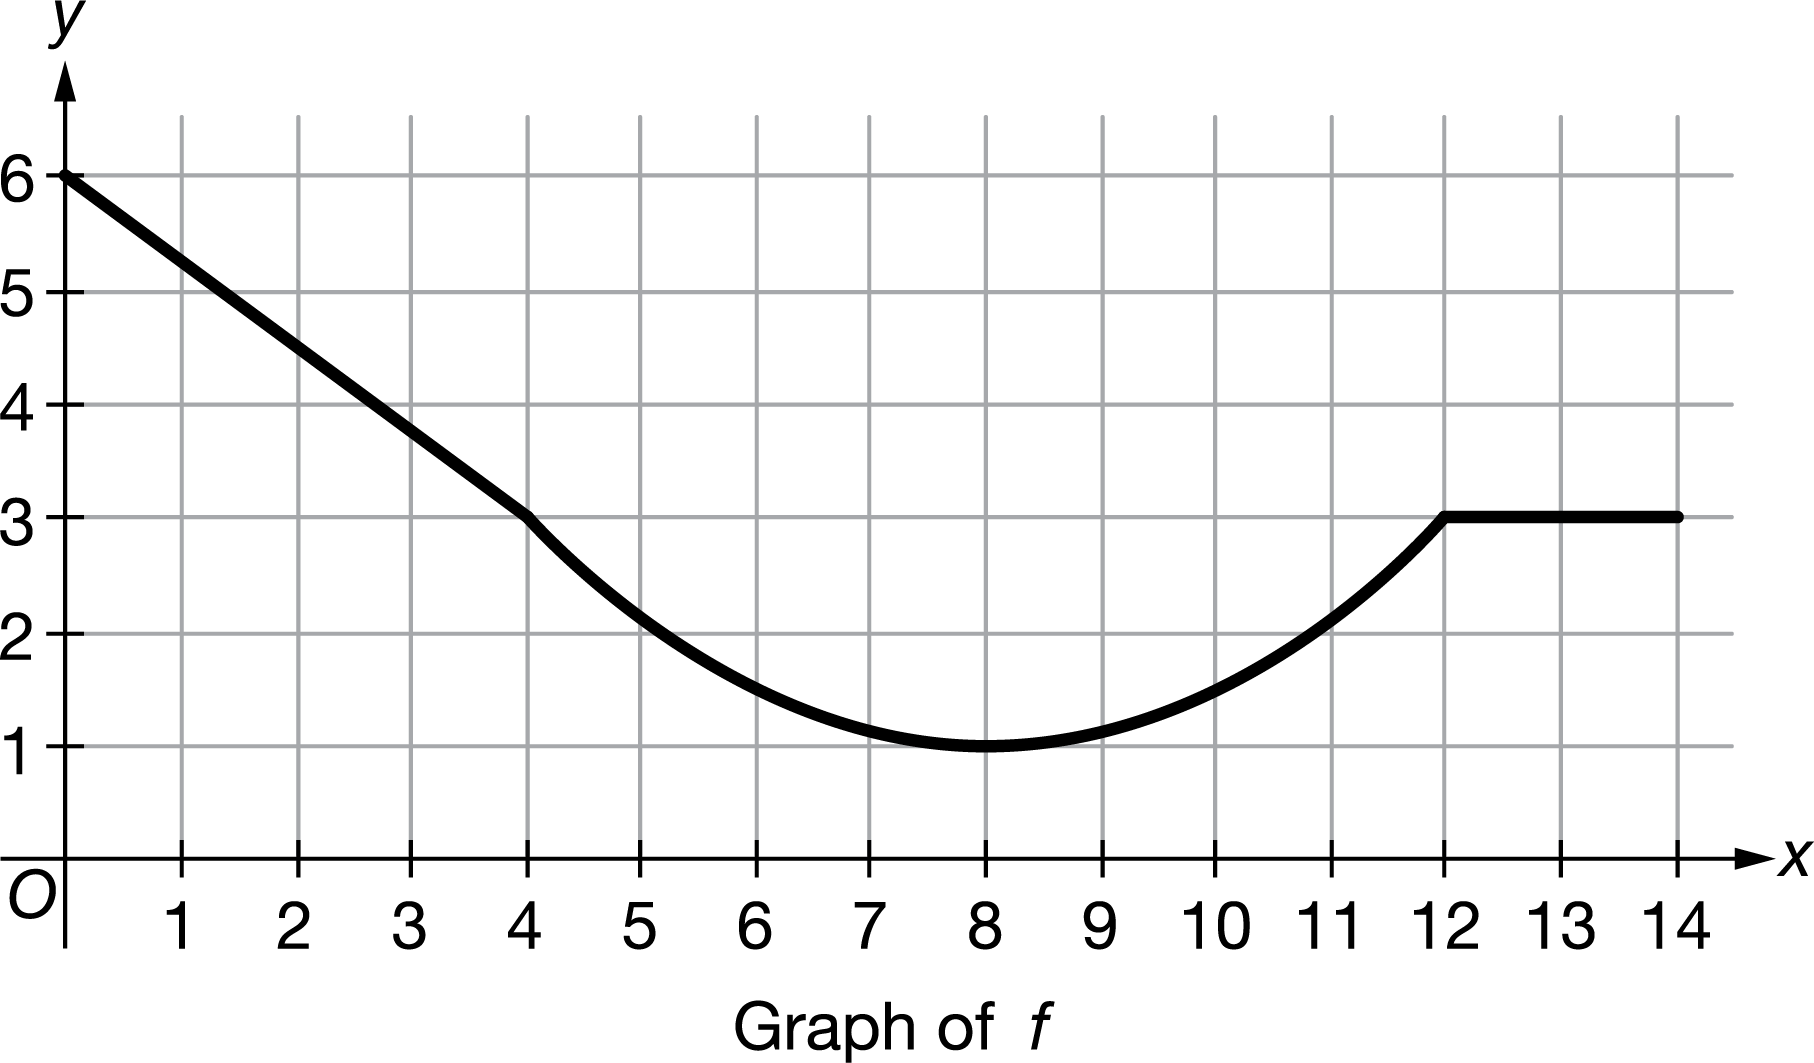
\includegraphics[width=3in]{4.041.png}
        \end{center}
\begin{equation*}
f(x) = 
\left\{
    \begin{array}{ll}
        6-\frac{3}{4}x & \text{for } 0 \leq x < 4 \\
        1+\frac{1}{8}(x-8)^2 & \text{for } 4 \leq x \leq 12 \\
       3 & \text{for } 12 \leq x \leq 14
    \end{array}
\right.
\end{equation*}
A skateboard track consists of a straight ramp followed by a curved section and a horizontal ledge. The track is modeled by the piecewise-defined function $f$ above, and the graph of $f$ is shown in the figure above. Which of the following expressions gives the total length of the track from $x=0$ to $x=14$?
        \begin{enumerate}
            \item
            \begin{equation*}
f'(x) = 
\left\{
    \begin{array}{ll}
        -\frac{3}{4} & \text{for } 0 \leq x < 4 \\
        \frac{1}{4}(x-8) & \text{for } 4 \leq x \leq 12 \\
       0 & \text{for } 12 \leq x \leq 14
    \end{array}
\right.
\end{equation*}
        \end{enumrate}
$$s=  \underbrace{\int_{0}^{4}\sqrt{1+\biggr(\frac{3}{4}\biggr)^2} \, dx}_{s_1} + \overbrace{\int_{4}^{12} \sqrt{1+ \bigg( \frac{1}{4}(x-8)\bigg)^2} \, dx}^{s_2} + \underbrace{\int_{12}^{14}\sqrt{1} \, dx}_{s_3} $$
\begin{enumerate}
    \item Using Pythagoras to find arc length when $x\in[0,4) \Longrightarrow s_1 = \sqrt{(3)^2+(4)^2}= 5$
    \item Using the trivial action of counting when $x\in(12,14] \Longrightarrow s_3 = 2$
\end{enumerate}
$$\boxed{s = 7 + \int_{4}^{12} \sqrt{1+ \frac{(x-8)^2}{16}} \, dx }$$
        \item The length of a curve from $x=1$ to $x=4$ is given by $\int_{1}^{4}\sqrt{1+9x^4} \, dx$. If the curve contains the point $(1,6)$, which of the following could be an equation for this curve?
$$\biggr(\frac{dy}{dx}\biggr)^2 = 9x^4 \xRightarrow[]{\text{Take square root}} \frac{dy}{dx} = 3x^2 \xRightarrow[]{\text{Integrate}} y=x^3+C \xRightarrow[]{\text{Evaluate using point}} C=5$$
$$\boxed{y=x^3+5}$$

\item Which of the following gives the length of the curve $y=\sqrt{x}$ over the closed interval $[1,4]$?
        \begin{enumerate}
            \item $y=\sqrt{x} \Longrightarrow \frac{dy}{dx} = \frac{1}{2\sqrt{x}}$
            \item $\big(\frac{dy}{dx}\big)^2 = \frac{1}{4x}$
        \end{enumerate}
        $$\boxed{s= \int_{1}^{4} \sqrt{1+\frac{1}{4x}} \, dx}$$
\end{enumerate}
\section*{4.05}
\begin{enumerate}
    \item At time $t=0$ years, a forest preserve has a population of 1500 deer. If the rate of growth of the population is modeled by $R(t)=2000e^{0.23t}$ deer per year, what is the population at time $t=3$?
\begin{enumerate}
    \item Let $P(t)$ denote the population of deer after time $t$ in years.
\end{enumerate}
$$P(3)=P(0)+\int_{0}^{3} R(t) \, dt = 1,500 + \int_{0}^{3} 2000e^{0.23t} \, dt \approx \boxed{10,141\text{ Deer}}$$
    \item A cup of tea is cooling in a room that has a constant temperature of 70 degrees Fahrenheit ($^\circ$F). If the initial temperature of the tea, at time $t=0$ minutes, is 200$^\circ$F and the temperature of the tea changes at the rate $R(t)=-6.89e^{-0.053t}$ degrees Fahrenheit per minute, what is the temperature, to the nearest degree, of the tea after 4 minutes?
\begin{enumerate}
    \item Let $T(t)$ denote the temperature of tea after time $t$ in minutes.
\end{enumerate}
$$T(4)=T(0)+\int_{0}^{3} R(t) \, dt = 200 - \int_{0}^{4} 6.89e^{-0.053t} \, dt \approx \boxed{175^\circ\text{F}}$$

    \item A spherical tank contains 81.637 gallons of water at time $t = 0$ minutes. For the next 6 minutes, water flows out of the tank at the rate of $9\sin\big(\sqrt{t+1} \big)$ gallons per minute. How many gallons of water are in the tank at the end of the 6 minutes?
    \begin{enumerate}
        \item Let $A(t)$ denote the amount of water after time $t$ in minutes.
    \end{enumerate}
    $$A(6)=81.637-\int_{0}^{6} 9\sin\big(\sqrt{t+1} \big) \, dt \approx \boxed{36.606 \text{ gallons}}$$

    \item The rate of change of the altitude of a hot-air balloon is given by $r(t) = t^2-4t^2+6$ for $0 \leq t \leq 8.$ Which of the following expressions gives the change in altitude of the balloon during the time the altitude is decreasing?
    \begin{enumerate}
        \item $r(t)<0$ when $t\in[1.572,3.514]$ 
    \end{enumerate}
    $$\boxed{\int_{1.572}^{3.514} r(t)\,dt}$$

    \item A city is built around a circular lake that has a radius of 1 mile. The population density of the city is $f(r)$ people per square mile, where $r$ is the distance from the center of the lake, in miles. Which of the following expressions gives the number of people who live within 1 mile of the lake?
    $$\boxed{2\pi\int_{1}^{2}r \cdot f(r) \, dr}$$

    \item A particle moves along a line so that its acceleration for $t \geq 0$ is given by $a(t)=\frac{t+3}{\sqrt{t^3+1}}$. If the particle’s velocity at $t=0$ is 5, what is the velocity of the particle at $t=3$?
    \begin{enumerate}
        \item Let $v(t)$ denote the velocity of the particle after time $t$.
    \end{enumerate}
    $$v(3)=v(0)+\int_{0}^{3} a(t) \, dt = 5 +\int_{0}^{3} \frac{t+3}{\sqrt{t^3+1}} \, dt \approx \boxed{11.710}$$

    \item A function $f(t)$ gives the rate of evaporation of water, in litres per hour, from a pond, where $t$ is measured in hours since 12 noon. Which of the following gives the meaning of $\int_{4}^{10} f(t) \, dt$ in the context described?
    $$\boxed{\text{The total volume of water, in litres, that evaporated from the pond between 16:00 and 22:00}}$$

    \item The temperature in a room at midnight is 20 degrees Celsius. Over the next 24 hours, the temperature changes at a rate modeled by the differentiable function $H$, where $H(t)$ is measured in degrees Celsius per hour and time $t$ is measured in hours since midnight. Which of the following is the best interpretation of $\int_{0}^{6} H(t) \, dt$?
$$\boxed{\text{The change in the temperature of the room, in degrees Celsius, between midnight and 06:00}}$$
    \item 
    \begin{center}
        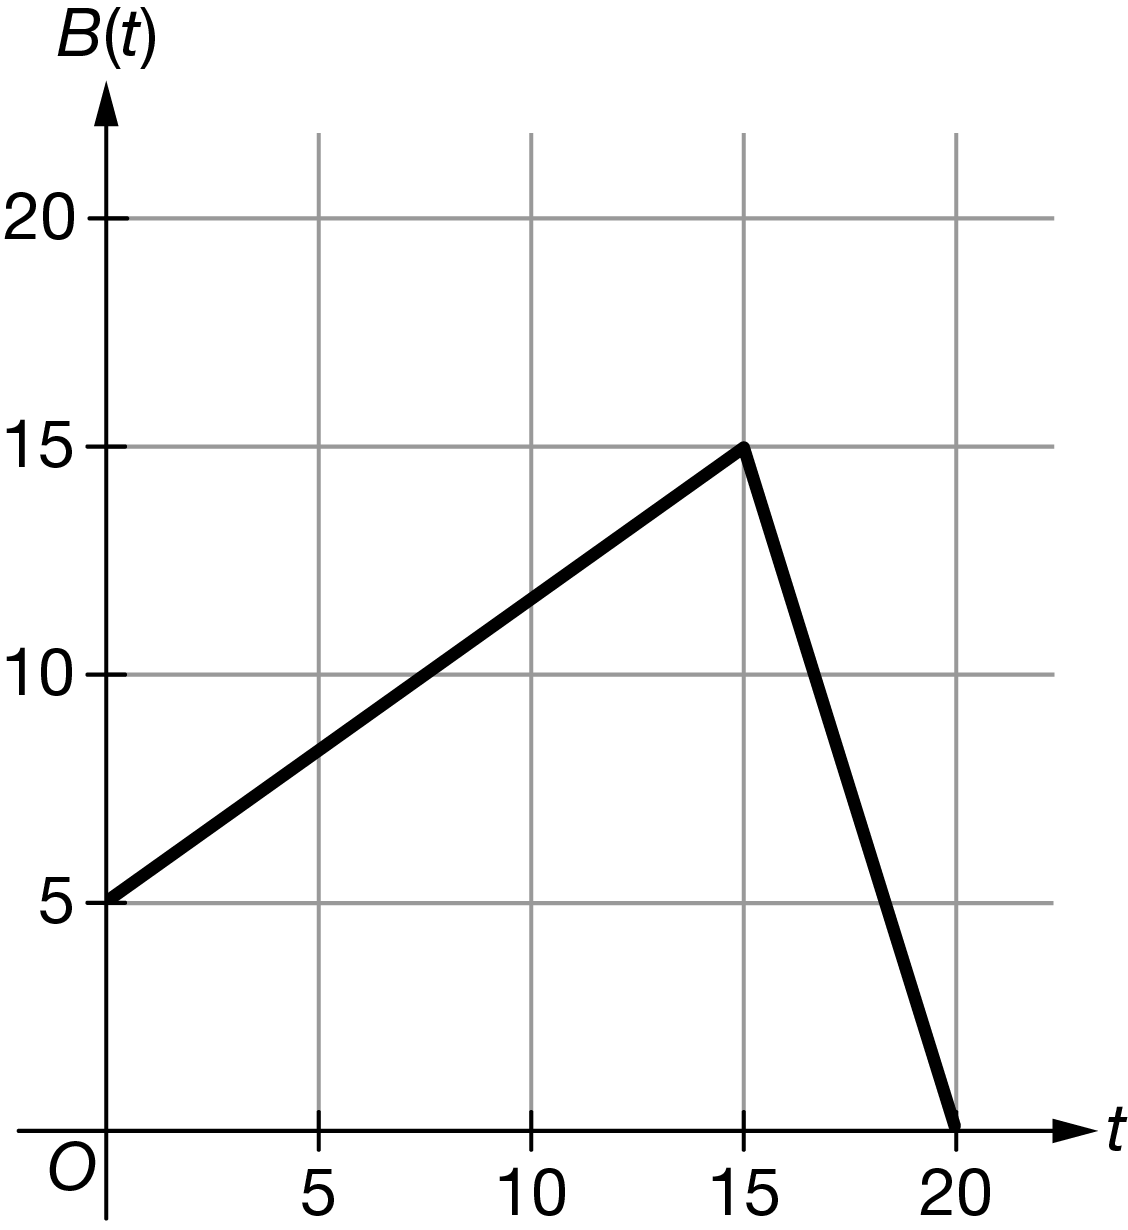
\includegraphics[width=2in]{4.051.png}
    \end{center}
    The rate at which people arrive at a theater box office is modeled by the function $B$, where $B(t)$ is measured in people per minute and $t$ is measured in minutes. The graph of $B$ for $0 \leq t \leq 20$ is shown in the figure above. Which of the following is closest to the number of people that arrive at the box office during the time interval $0 \leq t \leq 20$?
    $$\int_{0}^{20} B(t) \, dt = 187.5 \approx \boxed{188\text{ people}}$$

    \item Water is leaking from a dam during a particular week at a rate modeled by the function $F$ given by $F(t)=5+\frac{t}{4}-\sin \big(\frac{t^2}{5}\big)$, where $F(t)$ is measured in gallons per day and $t$ is the number of days since the start of the week on Sunday. How many gallons of water leak from the dam Tuesday through Thursday, days 2 through 4?
    $$\int_{2}^{4} F(t) \, dt \approx \boxed{10.010 \text{ gallons}}$$

    \item 
    \begin{center}
        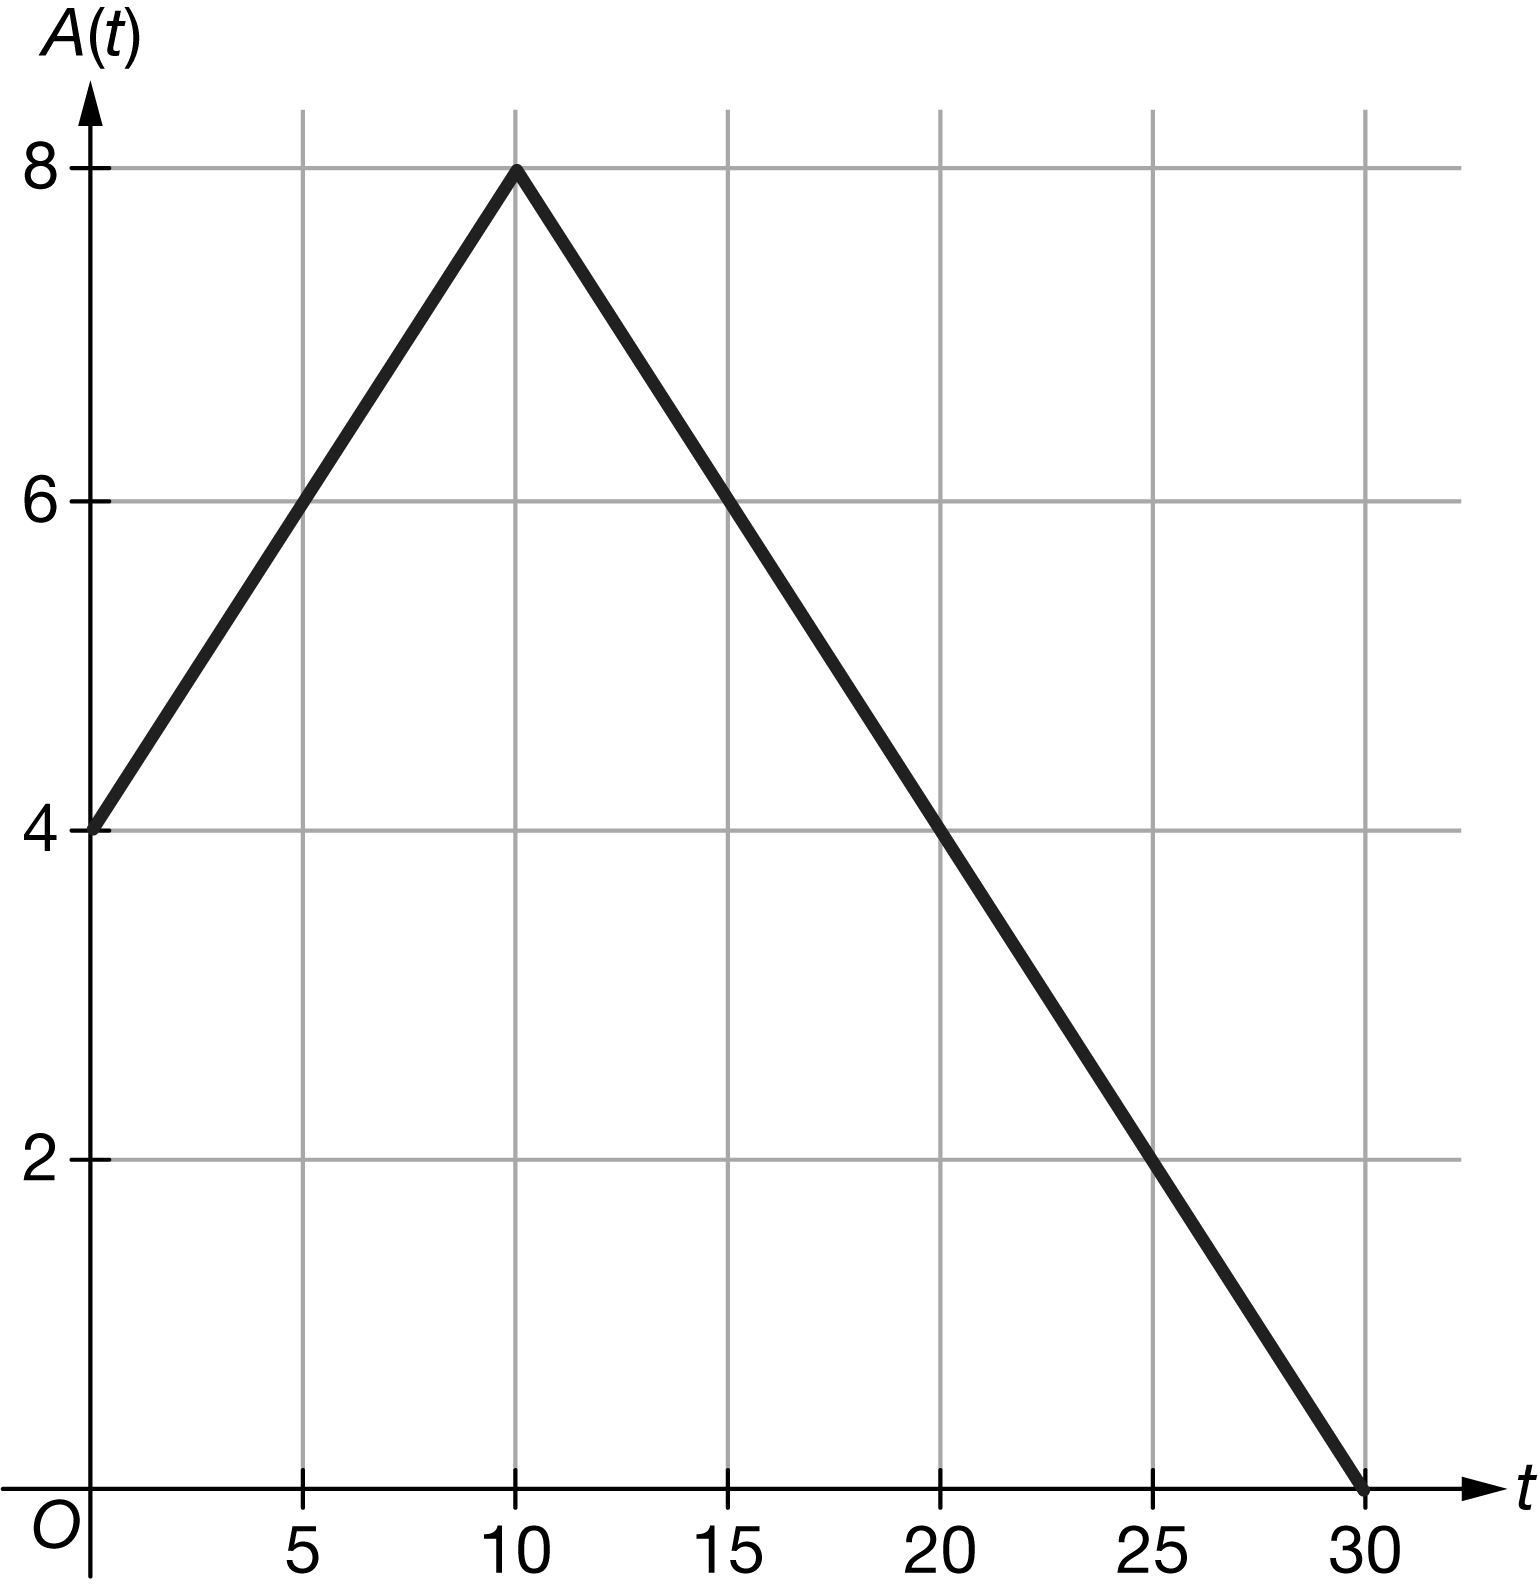
\includegraphics[width=2in]{4.052.png}
    \end{center}
    The rate at which ants arrive at a picnic is modeled by the function $A$, where $A(t)$ is measured in ants per minute and $t$ is measured in minutes. The graph of $A$ for $0 \leq t \leq 30$ is shown in the figure above. How many ants arrive at the picnic during the time interval $0 \leq t \leq 30$?
    $$\int_{0}^{3} A(t) \, dt = \boxed{140 \text{ Ants}}$$

    \item At time $t = 0$ minutes, a tank contains 48 gallons of water. For $0 \leq t \leq 4$ minutes, water flows into the tank at a rate of $E(t)=12t\sin\big(\frac{\pi t}{4}\big)$ gallons per minute, and water leaks out of the tank at a rate of $L(t)=\frac{6t^2}{t+2}$ gallons per minute. How many gallons of water are in the tank at time $t = 4$ minutes?
    \begin{enumerate}
        \item Let $A(t)$ denote the amount of water in the tank after time $t$ in minutes.
    \end{enumerate}
    $$A(4)=A(0) + \int_{0}^{4} \bigg(E(t)-L(t)\bigg) \, dt \approx \boxed{82.749 \text{ gallons}}$$

    \item The rate at which motor oil is leaking from an automobile is modeled by the function $L$ defined by $L(t) = 1 + \sin(t^2)$ for time $t \geq 0$. $L(t)$ is measured in litres per hour, and $t$ is measured in hours. How much oil leaks out of the automobile during the first half hour?
    $$\int_{0}^{0.5} \bigg(1+\sin(t^2)\bigg) \, dt \approx \boxed{0.541 \text{ litres}}$$

    \item Insects destroyed a crop at the rate of $\frac{100e^{-0.1t}}{20e^{-3t}}$ tons per day, where time $t$ is measured in days. To the nearest ton, how many tons did the insects destroy during the time interval $7 \leq t \leq 14$?
$$\int_{7}^{14} \frac{100e^{-0.1t}}{20e^{-3t}} \, dt \approx \boxed{125 \text{ tons}} $$
    \item A music group expects to sell a new compact disc (CD) at the rate $R(t)=20,000e^{-0.12t}$ CDs per week, where $t$ denotes the number of weeks since the CD was first released. To the nearest thousand, how many CDs are expected to be sold during the first 12 weeks after the release?
    $$\int_{0}^{12} R(t) \, dt \approx \boxed{127,000 \text{ compact discs}}$$
\end{enumerate}
\begin{center}
    
\includegraphics[width=2in]{Fleur de ise.jpg}
\end{center}
\end{document}